

% As a general rule, do not put math, special symbols or citations
% in the abstract
\subsection{Abstract}
Factorial Hidden Markov Models (FHMM) have emerged as a prominent modeling approach for energy disaggregation. However, because latent variables become dependent conditioned on the observation, reasoning about the posterior is usually intractable which is required for inference as well as learning. Recent approaches try to deal with these intractable posterior distributions by applying Variational Inference with an auxiliary distribution that assumes independence between latent states of the posterior. However, because posterior distributions in the context of energy disaggregation are often multi-modal, independent auxiliary distributions fail to capture \emph{either}-\emph{or} relationships between appliance states. In this paper, we introduce an auxiliary distribution over posterior states that, in principle, can approximate any multivariate Bernoulli distribution arbitrarily well, while at the same time offering a functional form that allows obtaining independent samples as well as the mode required for inference in $\mathcal{O}(N)$ where $N$ is the number of parallel Hidden Markov chains. On top of that, training the distribution requires solely samples of the joint distribution which are typically easy to acquire. We conduct experiments in the context of waveform disaggregation illustrating the superior capacity of the proposed distribution in comparison to independent auxiliary distributions trained on minimizing the forward or backward KL-divergence.


\subsection{Introduction}
Factorial Hidden Markov Model \cite{ghahramani1997factorial} (FHMM) are a natural choice for modeling the generative process of energy disaggregation~\cite{kolter2012fhmm,lange2016varbolt,ng2016scaling,hart1992}. FHMM are a generalization of Hidden Markov Models were multiple hidden chains evolve independently in parallel. Usually, the state of a single appliance is modeled by a single HMM chain, whereas the aggregate power measured at the main distribution panel is modeled by the aggregate observation. Let $z \in \mathcal{Z} = \{0,1\}^{N \times T}$ be the latent variable and $x \in \mathbb{R}^{S \times T}$ be the aggregate observation with $T$ number of time steps, $N$ number of parallel HMM chains and $S$ being the observation dimensionality. The joint distribution is defined as: \begin{align*}
p(x_{1:T},z_{1:T}) = \prod_t^T p(x_t|z_t)\prod_i^N p(z_{t,i}|z_{t-1,i})p(z_{0,i})
\end{align*} However, reasoning about the posterior of $P$ is usually difficult because the latent variables become conditionally dependent given the observation, specifically for the forward and filtering distribution hold respectively:
\begin{align}
p(x_{1:t},z_t) &= p(x_t|z_t) \sum_{z' \in \mathcal{Z}} p(z_t|z') p(z_{t-1}, x_{1:t-1}) \label{fnet:joint}\\
p(z_t|x_{1:t}) &= \frac{p(x_{1:t},z_t)}{\sum_{z' \in \mathcal{Z}} p(x_{1:t},z')} \label{fnet:post}
\end{align}
Note that (\ref{fnet:joint}) and (\ref{fnet:post}) both contain summations over $\mathcal{Z}$ and that the cardinality of $\mathcal{Z}$ grows exponentially with $N$.\\
\begin{figure}[!t]
\centering
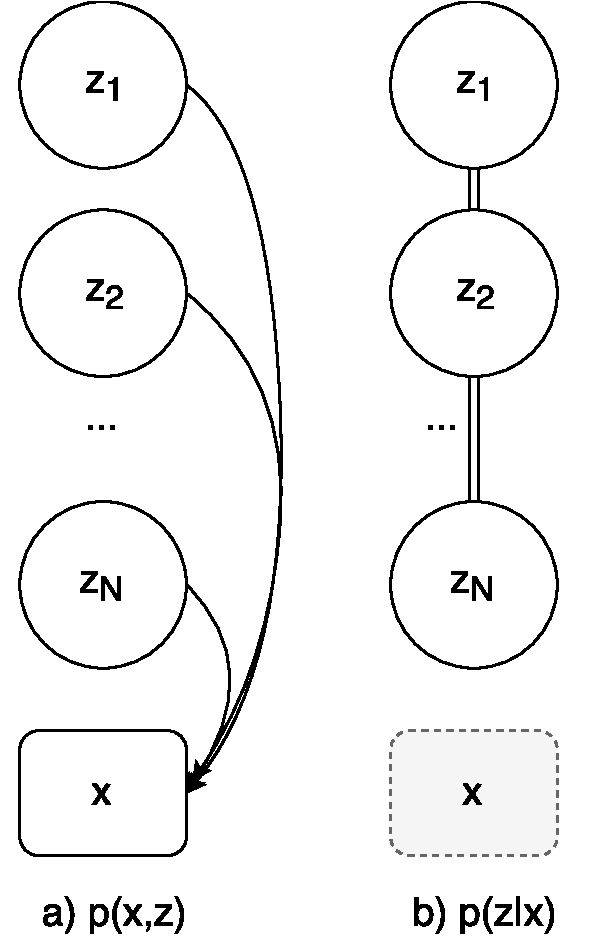
\includegraphics[width=0.4\linewidth]{factornet/graphmod.pdf}
% where an .eps filename suffix will be assumed under latex, 
% and a .pdf suffix will be assumed for pdflatex; or what has been declared
% via \DeclareGraphicsExtensions.
\caption[FactorNet: Latent variable models and independence structure.]{a) latent variables of the proposed distribution are marginally independent, however, become b) conditionally dependent given the observation}
\label{fnet:graphmod}
\end{figure}
Throughout this paper, for illustration, we will consider a slightly simpler distribution that nevertheless faces the same difficulty but for which exact solutions can be obtained and visualized for small $N$. Consider the graphical model that arises from removing the temporal dependencies between latent variables (Figure \ref{fnet:graphmod}a). Similar to FHMMs, latent variables become dependent conditioned on the observation $x$ (Figure \ref{fnet:graphmod}b). For the density holds: 
\begin{align}
p(x_{1:T},z_{1:T}) = \prod_t^T p(x_t, z_t) \label{fnet:factored}
\end{align}
As for FHMMs, the posterior of (\ref{fnet:factored}) is intractable, i.e. the number of states grows exponentially with the latent dimensionality rendering the denominator of the posterior intractable. However, previously, statistical tools such as Variational Inference \cite{jordan1999introduction} have been applied to reason about intractable posterior distributions in the context of energy disaggregation \cite{ng2016scaling,lange2016varbolt}. The main idea of Variational Inference is to introduce a tractable auxiliary distribution $Q_\psi$ parameterized by the variational parameters $\psi$. Inference is then turned into an optimization problem, i.e. $\psi$ is optimized in such a way that $Q$ best approximates $P$ as measured by the KL-divergence. Then, in order to perform inference on the intractable posterior $P$ inference can be carried out on $Q_\psi$ instead. Since $Q_\psi$ is required to be tractable, usually additional independence assumption are made and specifically, in the context of energy disaggregation, in order to deal with the difficulty of dependent latent variables, independence between latent states in the posterior is assumed. Note that $Q_\psi$ is usually required to be simpler than $P$, i.e. to have less capacity than $P$.\\
However, because inference is carried out on a simpler distribution, Variational Inference maximizes a lower bound on the data likelihood $p(x)$, i.e. it performs inference up to a constant and it can be shown that this constant is the KL divergence between $P$ and $Q_\psi$. Note also that because $Q$ is required to be simpler than $P$, the KL divergence usually never becomes 0.\\
Furthermore, if independence between latent states is assumed in $Q_\psi$, i.e. the posterior is factored as:
\begin{align}
q_\psi(z_{t}|x_{t}) = \prod_i f_\psi(x_t)_i^{z_i}(1-f_\psi(x_t)_i)^{1-z_i} \label{fnet:aux_dist}
\end{align}
with $f$ being bounded by $[0,1]$, $Q_\psi$ is often overly simple. It is easy to show that depending on whether the forward or backward KL divergence is employed as a divergence measure, the $Q$ introduced in (\ref{fnet:aux_dist}) either learns the mean or the mode of $P$. Specifically, for energy disaggregation, such a unimodal $Q$ is unable to learn \emph{either} this appliance \emph{or} the other.\\
Consider a scenario with 2 two-state appliances with comparable power draw and an aggregate observation $x'$ that is similar to the power consumption of each appliances. Thus we can assume that for the posterior the following holds:
\begin{align*}
p(z|x') &= \begin{pmatrix}
0&
0.5&
0.5&
0
\end{pmatrix}\\
 \text{with } z &=\begin{pmatrix} 0,0&
0,1 &
1,0 &
1,1 
\end{pmatrix}
\end{align*} Note that approaches that assume independence between latent states of the auxiliary distribution fail at capturing the \emph{either}-\emph{or} relationship between appliance states. Let $\psi^*_f$ and $\psi^*_b$ be optimal variational parameters that minimize the forward and backward KL-divergence between $P$ and $Q$ respectively. It can be shown that: 
\begin{align*}
q_{\psi^*_f}(z|x') = \begin{pmatrix}
0.25 &
0.25 &
0.25 &
0.25 
\end{pmatrix}\\
q_{\psi^*_b}(z|x') = \begin{pmatrix}
0 &
1 &
0 &
0 
\end{pmatrix}
\text{ or }
q_{\psi^*_b}(z|x') = \begin{pmatrix}
0 &
0 &
1 &
0 
\end{pmatrix}
\end{align*}
It is easy to see that independent of the choice of divergence measurement, $Q$ cannot capture a significant proportion of the information present in $P$, specifically the fact that one of the appliances is active but not both or none.\\
That is why we argue that previous approaches based on Variational Inference can be improved by a better choice of the auxiliary distribution. Thus, in this paper, we introduce a tractable auxiliary distribution $g$ that despite being tractable can approximate any discrete distribution arbitrarily well. To sum up, we propose an auxiliary distribution that has the following characteristics:
\begin{enumerate}
\item No independence assumptions and therefore unlimited capacity, i.e. in general, any multivariate Bernoulli distribution can be approximated arbitrarily well
\item The posterior can be trained efficiently based on samples of the joint $p(x,z)$
\item Computing the mode and drawing independent samples can be achieved in $\mathcal{O}(N)$
\end{enumerate}

In the next subsection we will provide a brief introduction into Variational Inference and introduce FactorNet, the proposed auxiliary distribution. We then conduct experiments in subsection 3 and conclude our findings.

\subsection{Variational Inference and FactorNet}

\begin{figure}
\centering
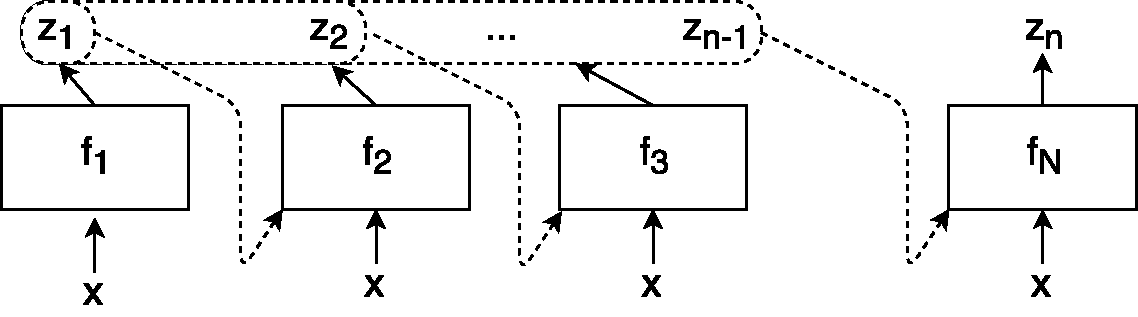
\includegraphics[width=0.9\linewidth]{factornet/factornet.pdf}
% where an .eps filename suffix will be assumed under latex, 
% and a .pdf suffix will be assumed for pdflatex; or what has been declared
% via \DeclareGraphicsExtensions.
\caption[FactorNet: A graphical depiction of the cascaded neural networks that factorize the joint probability distribution.]{A graphical depiction of the cascaded neural networks that factorize the joint probability distribution.}
\label{fnet:neuralnets}
\end{figure}

Variational Inference (VI) has experienced a recent surge in attention from various academic communities~\cite{hoffman2013stochastic,kingma2013auto}. One of the key advantages of VI over its alternatives such as Markov Chain Monte Carlo~\cite{geman1984stochastic} (MCMC) is speed. Since, as stated earlier, VI translates statistical inference into an optimization problem that produces a tractable distribution that best approximates the true posterior, inference can be amortized, i.e. time training the auxiliary distribution is spend once and after training, inference can be carried out extremely fast. This characteristic has direct implications in the context of energy disaggregation: VI-based approaches allow for inference on cheap hardware such as an electricity meter located in the premises whereas MCMC would require remotely collecting, storing and processing data. However, even in the asymptotic regime, VI is an approximate inference technique whereas (albeit slowly) MCMC is known to converge to the true posterior. The quality of the VI-based approximation crucially depends on the choice of the auxiliary distribution which can be seen when investigating the commonly used Evidence Lower Bound as the variational objective:
\begin{align}
\log p(x) &= \sum_z \log p(x|z) p(z)\\
              &= \sum_z \frac{q(z|x)}{q(z|x)} \log p(x|z) p(z)\\
              &\geq D_{KL} [q(z|x) || p(z)] + \mathbb{E}_{q(z|x)} [\log p(x|z)]
\end{align}
This inequality is tight if and only if $p(z|x) = q(z|x)$, however, this cannot be achieved when $Q$ is simpler than $P$. Furthermore note, that (7) is typically evaluated by Monte Carlo techniques, i.e. by evaluating the expectation by sampling from $Q$. Thus, in order for a Variational approach to be successful, $Q$ needs to be complex enough to be fit to $P$ tightly but simple enough to be sampled from efficiently.\\
For continuous distributions the problem of choosing a suitable posterior distribution has recently been addressed by introducing normalizing flows\cite{rezende2015variational}, i.e. a succession of invertible non-linear transformations of the random variable $z$. However, for discrete random variables this approach does not seem to be possible since the flow-operators are required to be differentiable but to be mapping into the same domain (in this case $\{0,1\}^N$). Or in other words, the flow-operator cannot at the same time be mapping into the discrete domain whilst being smooth and differentiable.\\
Furthermore, another difficulty that arises for VI-based approaches is the fact that the true posterior is usually not obtainable, thus all updates need to be made based on samples of the joint $p(x,z)$. Typically, this is circumvented by maximizing the variational objective (7), however, in the experience of the authors (7) has suboptimal convergence properties.\\
Thus, in this paper, we follow a different strategy. We directly learn the conditional factorization of the joint and show that once the joint is factorized, obtaining the posterior can be done efficiently. First, we note that any joint probability distribution can be factored according to the chain rule of probabilities:
\begin{align*}
p(z_{t}, x_{t}) &= p(z_{t,1},x_t)p(z_{t,2}, x_t|z_{t,1}) ... p(z_{t,N}, x_t| z_{t,N-1}, ..., z_{t,1})\\
		    &= \prod_n^N p(z_{t,n}, x_t|z_{t,1:n})
\end{align*}
The goal now is to learn this factorization. This is achieved by approximating every factor of the probability distribution by a neural network that takes the respective condition as input and produces the conditional joint probability. Thus, let $g$ be the FactorNet distribution and $f_n$ and $\overline{f}_n$ with $1 \leq n \leq N$ be the $N$ neural networks approximating the \emph{on} and \emph{off} factors of the joint distribution, i.e.:
\begin{align*}
f_i(x_t, z_1, ..., z_{i-1}) \approx p(x_t, z_{i} = 1 | z_1, ..., z_{i-1})\\
\overline{f}_i(x_t, z_1, ..., z_{i-1}) \approx p(x_t, z_{i} = 0 | z_1, ..., z_{i-1})\\
\end{align*}
therefore:
\begin{align*}
&p(z_i = 1 | x_t, z_1, ..., z_{i-1}) \\
\approx &\frac{f_i(x_t, z_1, ..., z_{i-1})}{f_i(x_t, z_1, ..., z_{i-1}) + \overline{f}_i(x_t, z_1, ..., z_{i-1})}\\
= &f^*_i(x_t, z_1, ..., z_{i-1})
\end{align*}
For the FactorNet joint distribution the following then holds:
\begin{align*}
g(z_{t}, x_{t}) = \prod_i^N &f_i(x_t, z_1, ..., z_{i-1})^{z_i} \\
			& \overline{f}_i(x_t, z_1, ..., z_{i-1})^{(1-z_i)}
\end{align*} 
and for its posterior:
\begin{align*}
g(z_{t}| x_{t}) = \prod_i^N &f^*_i(x_t, z_1, ..., z_{i-1})^{z_i} \\
			&(1- f^*_i(x_t, z_1, ..., z_{i-1}))^{(1-z_i)}
\end{align*} 
Note that because the joint instead of the posterior probability is factorized, $f_i(x_t, z_1, ..., z_{i-1}) + \overline{f}_i(x_t, z_1, ..., z_{i-1}) \neq 1$ and that even though no independence assumption between latent variables has been made, evaluating the joint as well as the posterior probability is linear in the latent dimensionality as opposed to exponential for evaluating $P$. Furthermore, we can take independent samples from the posterior of $G$ efficiently, i.e. linear time. That is, we do not have to resort to Markov Chain Monte Carlo techniques for drawing samples from $g$, which would, in principle, allow for an efficient Monte Carlo approximation of the expectation of (7) given the samples from $Q$. See Algorithm 1 for how to sample from $g(z|x)$.

\begin{algorithm}
 \KwResult{Sample or Mode of $g(z|x_t)$ }
 $z = \{\}$\;
 \For{$n = 1, ..., N$}{
  $p_n = f_n(x_t, z)/(f_n(x_t, z) + \overline{f}_n(x_t, z))$\;
  \eIf{$p_n > threshold$}{
   Append $1$ to $z$
   }{
   Append $0$ to $z$\;
  }
 }
 \caption{Outputs either an independent sample or the mode of $g(z|x_t)$. If the mode is desired, set $threshold = 0.5$ and to a sample from $g(z|x_t)$ set $threshold \sim U[0,1]$, i.e. to a sample from a uniform distribution.}
\end{algorithm}

However, as stated above, (7) has suboptimal convergence properties that can be circumvented by exploiting the fact that $G$ allows to efficiently obtain the joint as well as the posterior. That is why we propose a learning objective that directly minimizes the KL-divergence between the joint distributions, i.e.:
\begin{align*}
\mathcal{L} = -g(z_t, x_t) \log \frac{p(z_t, x_t)}{g(z_t, x_t)}
\end{align*}
Note that we do not allow the gradients to flow into the fraction, i.e. we treat $g(z_t, x_t)$ in the denominator as a constant.

\subsection{Experiments}

\begin{figure}
\centering
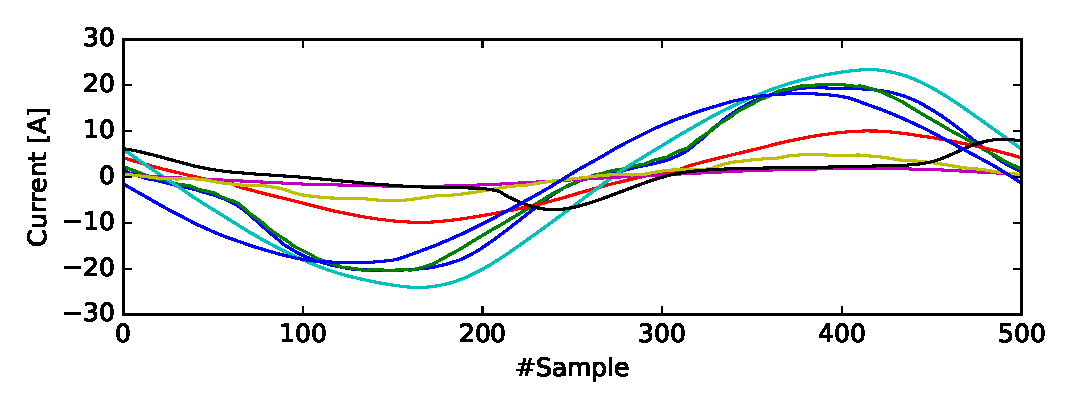
\includegraphics[width=0.9\linewidth]{factornet/waveforms.pdf}
% where an .eps filename suffix will be assumed under latex, 
% and a .pdf suffix will be assumed for pdflatex; or what has been declared
% via \DeclareGraphicsExtensions.
\caption[FactorNet: The current waveforms used in the synthetic experiment taken from PLAID datasets.]{The current waveforms used in the synthetic experiment taken from PLAID datasets. Current waveforms were extracted by alignment to zero-crossings in the voltage line.}
\label{fig_waveforms}
\end{figure}

The efficacy of FactorNet is evaluated on a synthetic experiment in the context of supervised waveform disaggregation. Specifically, we choose 8 appliances from the PLAID dataset\cite{gao2014plaid} and extract a single steady-state current waveform for every appliance aligned by zero-crossing of the voltage line. PLAID is a publicly available dataset containing high-frequency current and voltage measurements of single appliances. Since PLAID is collected at 30kHz, approximately 500 samples are collected per voltage cycle. Thus a matrix $W\in \mathbb{R}^{500\times8}$ was extracted from PLAID and Figure \ref{fig_waveforms} shows the waveforms used in the experiments. The 8 appliance waveforms were then mixed up, i.e. all 256 possible combinations of waveforms were created and corrupted by Gaussian noise: $X = \{Wz + \mathcal{N}(0, 0.1 I) | z \in \{0,1\}^8\}$. The probability of the aggregate observation was defined as:
\begin{align*}
p(x_t|z_t) = \mathcal{N}(x_t | Wz_t, 0.1 I)
\end{align*}
with $W$ being a matrix containing the appliance waveforms and $I$ being the identity matrix.
For the posterior thus holds:
\begin{align*}
p(z_t|x_t) = \frac{\mathcal{N}(x_t | Wz_t, 0.1 I)}{\sum_z \mathcal{N}(x | Wz, 0.1 I)}
\end{align*}
\begin{figure}
\centering
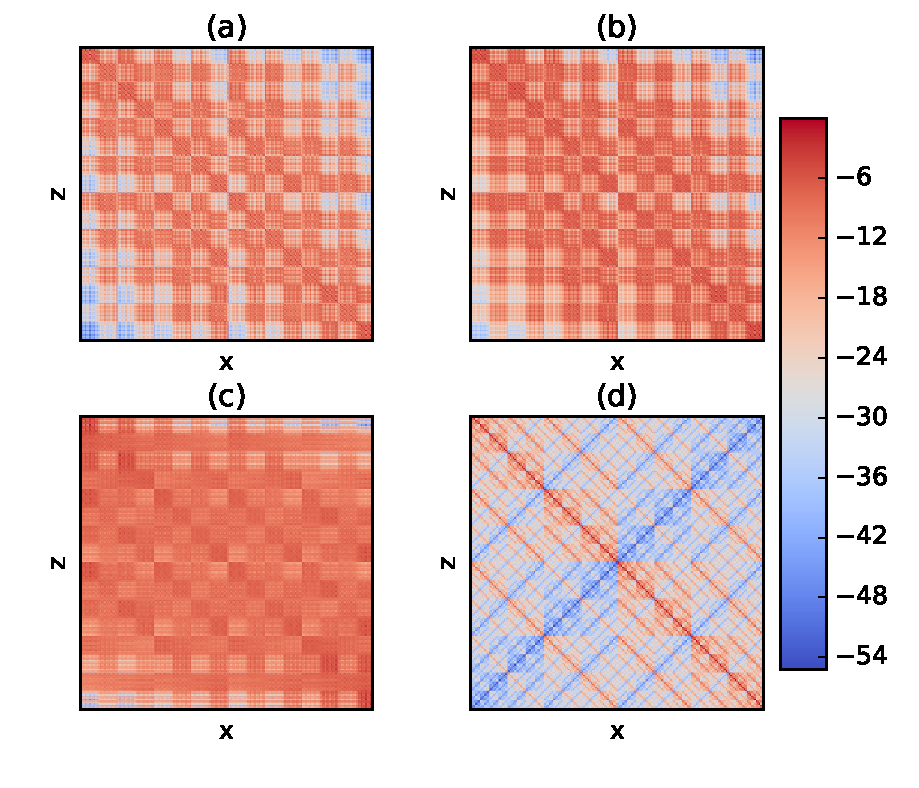
\includegraphics[width=0.9\linewidth]{factornet/posteriors2.pdf}
% where an .eps filename suffix will be assumed under latex, 
% and a .pdf suffix will be assumed for pdflatex; or what has been declared
% via \DeclareGraphicsExtensions.
\caption[FactorNet: Performance comparison.]{(a) The true posterior $\log p(z|x)$ (b) The FactorNet posterior $\log g(z|x)$ (c) The posterior $\log q(z|x)$ minimizing the forward KL-divergence (d) The posterior $\log q(z|x)$ minimizing the backward KL-divergence. Note that all probabilities were clipped between 0.001 and 0.999 to avoid $\log(0)$}
\label{fig_posteriors}
\end{figure}

For every combination of $z \in \{0,1\}^8$ and $x \in X$, $\log p(z|x)$ was computed and stored. See Figure \ref{fig_posteriors}(a) for a plot of the resulting $256 \times 256$ matrix.\\
Eight neural networks with a similar topology were created with an input dimensionality of $500 + (n-1)$, two intermediate \emph{relu}-layers with 512 hidden units and two-unit \emph{sigmoid} output-layer for $f$ and $\overline{f}$ respectively. The network was trained by minimizing $\mathcal{L}$ introduced earlier. The objective was minimized by drawing mini-batches of 144 samples uniformly from the joint distribution $p(z,x)$. The training procedure did not assume knowledge of the posterior $p(z|x)$ and was solely presented with sampled of the joint. The performance of the algorithm is compared to distributions $q_{\psi^*_f}$ and $q_{\psi^*_b}$ introduced earlier, i.e. distributions that assume independence between latent states in the posterior and minimize the forward and backward KL-divergence respectively. The parameters $\psi^*_f$ and $\psi^*_b$ were obtained with the knowledge of the true posterior that usually is not available, thus we compare to distributions in their globally optimal configuration.\\
Figure \ref{fig_posteriors} shows a visual comparison of the different resulting posterior distributions. One can see that FactorNet $G$ captures much more information present in $P$ compared to $Q$ in both settings. Figure \ref{fig_epochs} emphasizes this fact as it shows the KL-divergence over time. One can see that FactorNet reaches a KL-divergence of practically 0 after approximately 100 iterations.

\begin{figure}
\centering
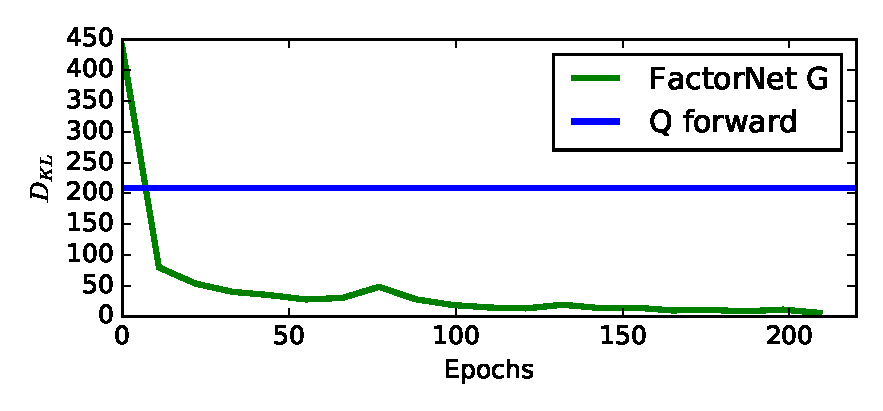
\includegraphics[width=0.9\linewidth]{factornet/epochs.pdf}
% where an .eps filename suffix will be assumed under latex, 
% and a .pdf suffix will be assumed for pdflatex; or what has been declared
% via \DeclareGraphicsExtensions.
\caption[FactorNet: KL-divergence as a function of learning epochs]{The KL-divergence $D_{KL}(p(z|x) || f(z|x))$ summed over all $x$. In this case $f$ is either the FactorNet distribution $g$ or the $q_{\psi^*_f}$ minimizing the forward KL divergence. Note that $q_{\psi^*_b}$ minimizing the backward KL divergence did not fit onto the plot with a divergence of approximately $3800$.}
\label{fig_epochs}
\end{figure}



% An example of a floating figure using the graphicx package.
% Note that \label must occur AFTER (or within) \caption.
% For figures, \caption should occur after the \includegraphics.
% Note that IEEEtran v1.7 and later has special internal code that
% is designed to preserve the operation of \label within \caption
% even when the captionsoff option is in effect. However, because
% of issues like this, it may be the safest practice to put all your
% \label just after \caption rather than within \caption{}.
%
% Reminder: the "draftcls" or "draftclsnofoot", not "draft", class
% option should be used if it is desired that the figures are to be
% displayed while in draft mode.



% Note that the IEEE typically puts floats only at the top, even when this
% results in a large percentage of a column being occupied by floats.


% An example of a double column floating figure using two subfigures.
% (The subfig.sty package must be loaded for this to work.)
% The subfigure \label commands are set within each subfloat command,
% and the \label for the overall figure must come after \caption.
% \hfil is used as a separator to get equal spacing.
% Watch out that the combined width of all the subfigures on a 
% line do not exceed the text width or a line break will occur.
%
%\begin{figure*}[!t]
%\centering
%\subfloat[Case I]{\includegraphics[width=2.5in]{box}%
%\label{fig_first_case}}
%\hfil
%\subfloat[Case II]{\includegraphics[width=2.5in]{box}%
%\label{fig_second_case}}
%\caption{Simulation results for the network.}
%\label{fig_sim}
%\end{figure*}
%
% Note that often IEEE papers with subfigures do not employ subfigure
% captions (using the optional argument to \subfloat[]), but instead will
% reference/describe all of them (a), (b), etc., within the main caption.
% Be aware that for subfig.sty to generate the (a), (b), etc., subfigure
% labels, the optional argument to \subfloat must be present. If a
% subcaption is not desired, just leave its contents blank,
% e.g., \subfloat[].


% An example of a floating table. Note that, for IEEE style tables, the
% \caption command should come BEFORE the table and, given that table
% captions serve much like titles, are usually capitalized except for words
% such as a, an, and, as, at, but, by, for, in, nor, of, on, or, the, to
% and up, which are usually not capitalized unless they are the first or
% last word of the caption. Table text will default to \footnotesize as
% the IEEE normally uses this smaller font for tables.
% The \label must come after \caption as always.
%
%\begin{table}[!t]
%% increase table row spacing, adjust to taste
%\renewcommand{\arraystretch}{1.3}
% if using array.sty, it might be a good idea to tweak the value of
% \extrarowheight as needed to properly center the text within the cells
%\caption{An Example of a Table}
%\label{table_example}
%\centering
%% Some packages, such as MDW tools, offer better commands for making tables
%% than the plain LaTeX2e tabular which is used here.
%\begin{tabular}{|c||c|}
%\hline
%One & Two\\
%\hline
%Three & Four\\
%\hline
%\end{tabular}
%\end{table}


% Note that the IEEE does not put floats in the very first column
% - or typically anywhere on the first page for that matter. Also,
% in-text middle ("here") positioning is typically not used, but it
% is allowed and encouraged for Computer Society conferences (but
% not Computer Society journals). Most IEEE journals/conferences use
% top floats exclusively. 
% Note that, LaTeX2e, unlike IEEE journals/conferences, places
% footnotes above bottom floats. This can be corrected via the
% \fnbelowfloat command of the stfloats package.




\subsection{Conclusion}
We introduced an auxiliary distribution capable of approximating any multivariate Bernoulli distribution arbitrarily well whilst at the same time having a functional form that is simple enough to allow for drawing samples as well as computing the mode of the posterior efficiently. The joint as well as posterior distribution can be obtained in linear time by approximating the chain rule factorization through a succession of neural networks, which allows for using a training objective that minimizes the divergence between the joint distributions directly circumventing the need for ELBO minimization. Positive experimental results of the performance were obtained in the setting of supervised waveform disaggregation.\\
However, experiments in which FactorNet incorporates temporal dependencies have not yet been conducted. Note that FactorNet was conceived out of the realization that auxiliary distributions that assume independence in the posterior are detrimental when modeling temporal dependencies, i.e. the posterior collapses onto a single state and most of the uncertainty is falsely explained away. This prohibits temporal models from reversing previous decisions like e.g. the Viterbi~\cite{viterbi1967error} algorithm would. FactorNets performance with temporal dependencies needs yet to be determined.


